\section{Implementation}
\label{impl}

Um einen Eindruck der hashbasierten Inversionsmethode und ihrer Arbeitsweise zu bekommen, 
wird jetzt eine konkrete Implementierung dieser angesprochen und Ergebnisse bei 
unterschiedlichen Eingaben gezeigt. Geschrieben wurde das Programm in Python mithilfe der 
Pakete \textit{numpy} und \textit{matplotlib}.

Schretter \cite{schretter-golden_ratio_sequences-2012} stellt am Ende der Arbeit eine 
C++-Methode zur Generierung einer zweidimensionalen Goldenen-Schnitt-Sequenz zur Verfügung. 
Diese Methode wurde in ein Python-Script übertragen und alle, in diesem Kapitel erwähnte, zufällige, uniformen
Variablen $U$ werden mit diesem Script generiert.
\begin{figure}
    \centering
    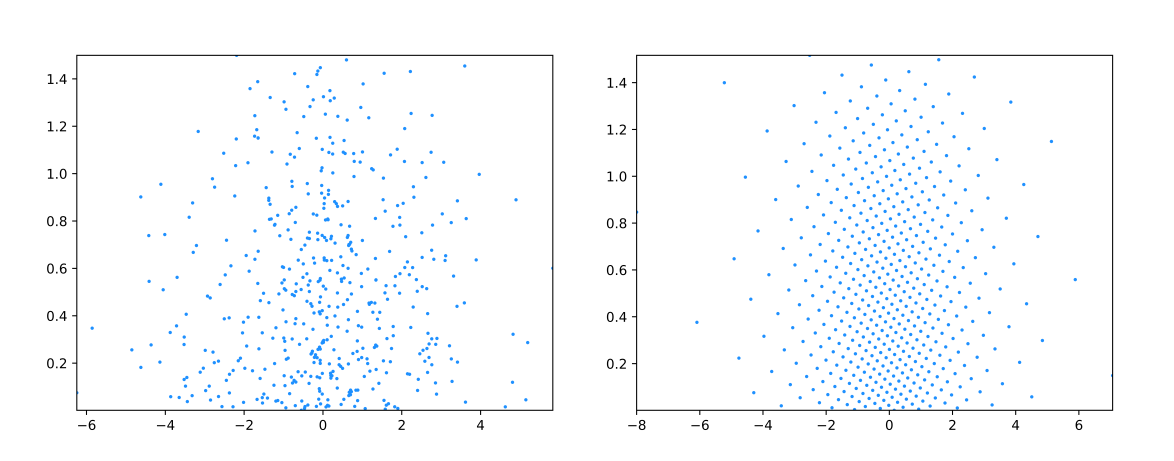
\includegraphics[width=0.48\textwidth]{fig2.png}
    \caption{500 Punkte mit einer logistischen Dichte auf der X- und sinusoider auf der Y-Achse 
            (a) Ursprungspunkte zufällig mit \code{random} (b) Ursprungspunkte aus einer Golden Ratio Sequence.}
    \label{bild:grs-vs-rnd}
\end{figure}

Zum Testen der vorgestellten Methode wurde das Konzept von Chen und Asau \cite{chen_asau-generating_random_variates-1974} 
implementiert. Dabei wurde kein großer Wert auf optimale Laufzeiten gelegt, sondern darauf, eine Demonstration 
des Verfahrens geben zu können.

% TODO
% Ergebnisse bei unterschiedlichen Werten auswerten nicht nur im Bild
\dots


